
Рентгеновское излучение, взаимодействуя с электронами атомов вещества рассеивается.
Протоны (ядра атомов) в рассеянии рентгеновских лучей практически не участвуют, т.к.
амплитуда электромагнитной волны, рассеянной заряженной частицей,
 обратно пропорциональна ее массе - формула Томсона \cite{iveronova1972}. Величина такого рассеяния
 зависит от количества электронов в атоме.  Тяжелые металлы,
 например свинец, Pb (Z = 82), рассеивают рентгеновское излучение сильнее легких,
 таких как Ni (Z = 28) или  Co (Z = 27), а такие атомы, как He или H – прозрачны
 для рентгеновского излучения. Определим атомный множитель $f$ (атомный фактор рассеяния)
как отношение амплитуды волны, рассеянной одним атомом, к амплитуде волны, рассеянной
одним свободным электроном. Действительно, если в какой либо точке пространства сосредоточено
$Z$ электронов, то заряд этой группы равен $Q = Z\cdot e$, а масса $M = Z \cdot m_e$.

На рисунке ~\ref{ris:atom_factor} представлена диаграмма направленности атомного
фактора лантана в зависимости от угла. Размеры атома соизмеримы с длиной волны
рентгеновских лучей, поэтому между волнами рассеянными отдельными электронами, возникает
разность фаз. Это разность фаз равна нулю только при $2 \theta = 0$, поэтому структурный
фактор зависит от $\theta$ и $\lambda$. Максимальная величина, которая равна $Z$,
 наблюдается в случае рассеяния вперед и рассеяния назад.

\begin{figure}[H]
  \centering
  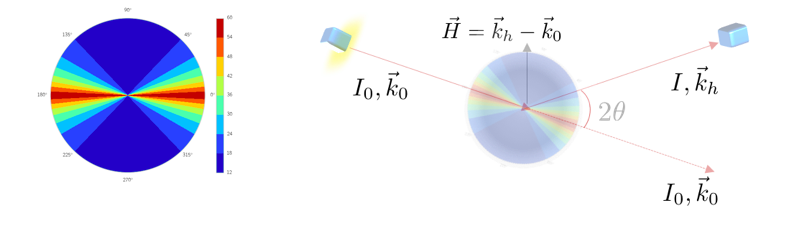
\includegraphics[width=0.9\textwidth]{images/atom_factor.png}
  \caption{ (Слева) фактор рассеяния для атома лантана (La, N = 57), (справа)
  схема расположения векторов для падающей и рассеянной волн}
  \label{ris:atom_factor}
\end{figure}

Приближенное выражение для расчета атомного фактора рассеяния
представляется \cite{International_Tables} в виде выражения:

\begin{equation}
  f_0 = \sum_{i=1}^{4} \cdot a_i e^{ -b_i (\frac{sin \vartheta_B}{\lambda})^2} + C
 \end{equation}
где $a_i$, $b_i$ и $c$ - коэффициенты Кромер-Манна для бездисперсионного канала рассеяния атомами решетки,
ограничением является $0<\frac{sin\vartheta}{\lambda}<2.0 \angstrom ^{-1}$.
 Характерная зависимость структурного фактора от угла рассеяния и длины волны
для атомов входящих в состав кристалла LGT (La, Ga, Ta, O) представлена на рисунке ~\ref{ris:atom_factor_GaLaTa}.

\begin{figure}[H]
  \centering
  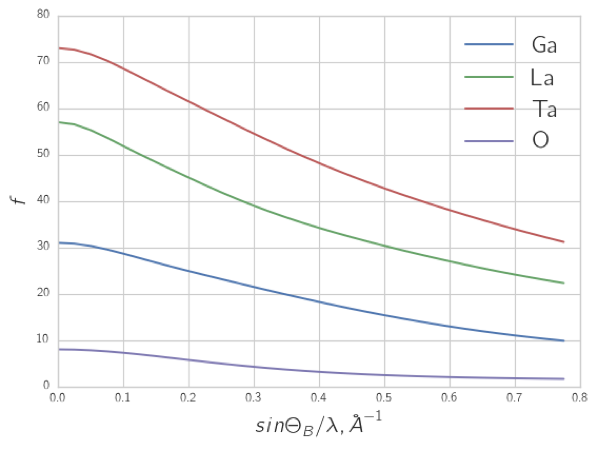
\includegraphics[width=0.6\textwidth]{images/atom_factor_GaLaTa.png}
  \caption{ Атомный фактор рассеяния для атомов: галлия (Ga), лантана (La), тантала (Ta) и  кислорода (O)}
  \label{ris:atom_factor_GaLaTa}
\end{figure}

При расчете интенсивности рассеяния атомом необходимо учитывать факт,
что все электроны связаны между собой, таким образом необходимо записывать
уравнение движение связанного электрона по действием падающего излучения \cite{iveronova1972}.
Если атом многоэлектронный, то амплитуда рассеянной волны равна сумме амплитуд волн,
рассеянных всеми электронами атома:

\begin{equation}
  f = f_0 + f^{'} + i f^{''}
 \end{equation}

 где, $f_0$ - атомный фактор рассеяния, рассчитанный без учета сил связи электронов
 с ядром, а $f^{'}$ и $f^{''}$ - дисперсионные поправки \cite{f0f1f12},
 первая из которых учитывает дополнительное рассеяние,
а вторая - дополнительное поглощение вблизи собственных частот колебаний электронов в атоме.

 \begin{figure}[H]
   \centering
   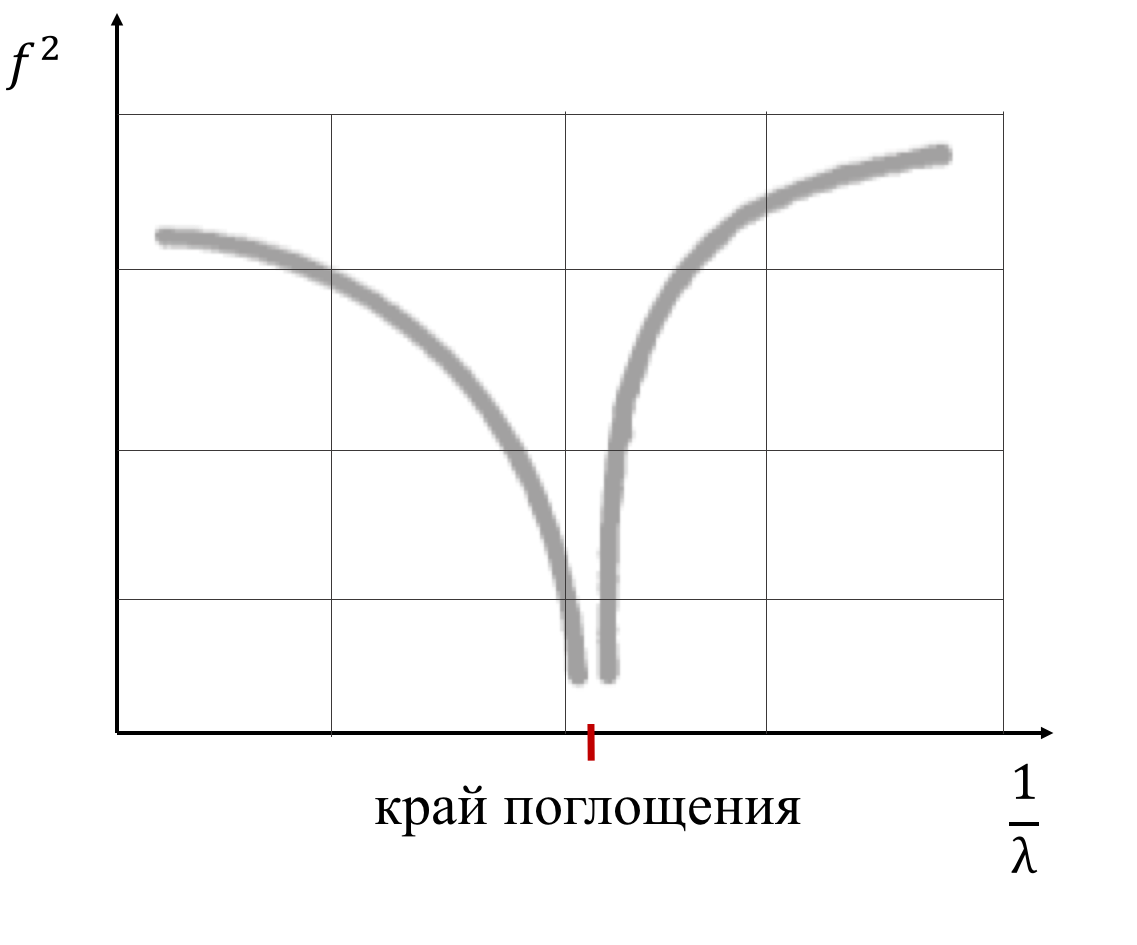
\includegraphics[width=0.4\textwidth]{images/dispers_f.png}
   \caption{ Схематичная зависимость атомного фактора $f^2 = (f_0 + f^{'})^2 + (f^{''})^2 $ от
   длины волны $\lambda$ вблизи края поглощения}
   \label{ris:dispers_f}
 \end{figure}

Дисперсионные поправки зависят от длины волны и практически не зависят
от $\theta$. А так как $f_0$ уменьшается с ростом угла рассеяния,
 дисперсионные поправки начинают играть роль при больших углах рассеяния.
